\documentclass[a4paper]{SIGCOMM}


\usepackage{tkz-orm}
\usepackage{hyperref}
\usepackage[utf8x]{inputenc}
\usepackage[T1]{fontenc}
\usepackage{lmodern}
\usepackage{fullpage}
\usepackage{graphicx}
\usepackage{epstopdf}
\usepackage{caption}
\usepackage{subcaption}
\usepackage{multirow}
\usepackage{framed}
\usepackage{eurosym}
\usepackage{multicol}
\usepackage{url}
\usepackage{attrib}

\usepackage{arydshln}


%Caractères spéciaux
\usepackage{pifont}
\usepackage[margin=2cm]{geometry}

% Affichage du graphique
\usepackage{tikz}
\usetikzlibrary{shapes, decorations.markings, shadows, arrows, positioning}
\usepackage{xcolor}

%inclure du code
\usepackage{listingsutf8}

% cfr http://en.wikibooks.org/wiki/LaTeX/Colors
\usepackage{color}
\usepackage{colortbl}
%\usepackage[usenames,dvipsnames,svgnames,table]{xcolor}
\definecolor{dkgreen}{rgb}{0.25,0.7,0.35}
\definecolor{dkred}{rgb}{0.7,0,0}

\usepackage{float}
\usepackage{pict2e}
\usepackage[noadjust]{cite}
\usepackage{listings}
\lstset{
  numbers=left,
  numberstyle=\tiny\color{gray},
  basicstyle=\rm\small\ttfamily,
  keywordstyle=\bfseries\color{dkred},
  frame=single,
  commentstyle=\color{gray}=small,
  stringstyle=\color{dkgreen},
  %backgroundcolor=\color{gray!10},
  %tabsize=2,
  rulecolor=\color{black!30},
  %title=\lstname,
  breaklines=true,
  framextopmargin=2pt,
  framexbottommargin=2pt,
  extendedchars=true,
  inputencoding=utf8x
}

\lstset{language={C}}

\hypersetup{
    % pdfborder={0 0 0}
}

\begin{document}

% Table of contents depth

\title{Reproducibility}

\author{\begin{tabular}{c}Bonaventure Olivier\\ olivier.bonaventure@uclouvain.be \end{tabular} 
\and \begin{tabular}{c}Houtain Nicolas \\ nicolas.houtain@student.uclouvain.be \end{tabular} }
\date{\date}

\maketitle

\begin{abstract}
%TODO
\end{abstract}


\section{Intro}

\section{Result}

\begin{figure*}[!t]
    \centering
    \begin{tabular}{p{0.7\columnwidth}p{0.7\columnwidth}p{0.7\columnwidth}}
    \href{http://nhoutain.github.io/Reproducibility/}
        {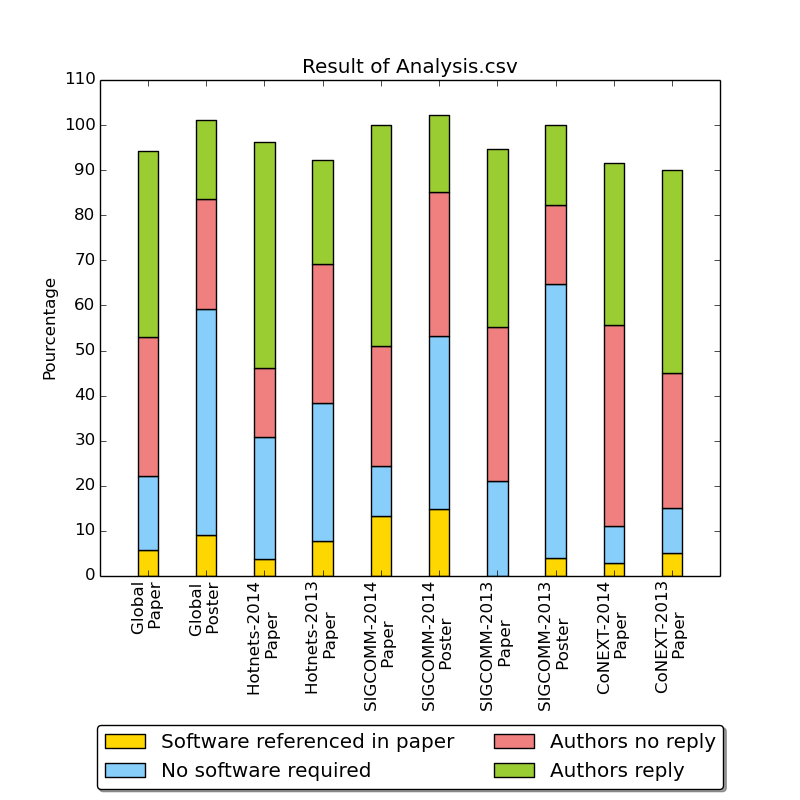
\includegraphics[width=0.7\columnwidth]{stat/global-analysis.png}} &

    \href{http://nhoutain.github.io/Reproducibility/}
        {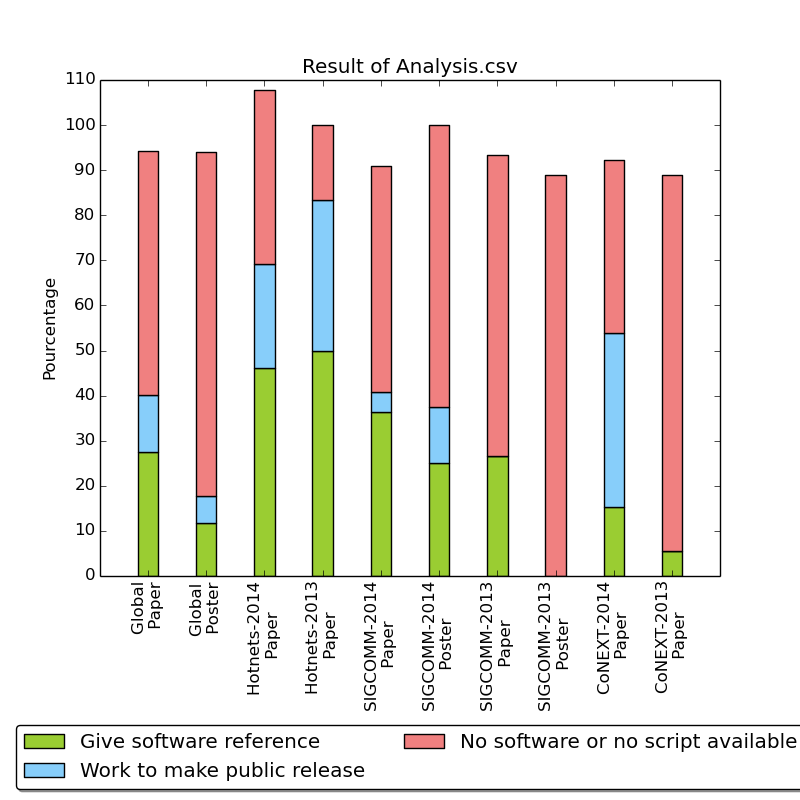
\includegraphics[width=0.7\columnwidth]{stat/mail-analysis.png}} &

    \href{http://nhoutain.github.io/Reproducibility/}
        {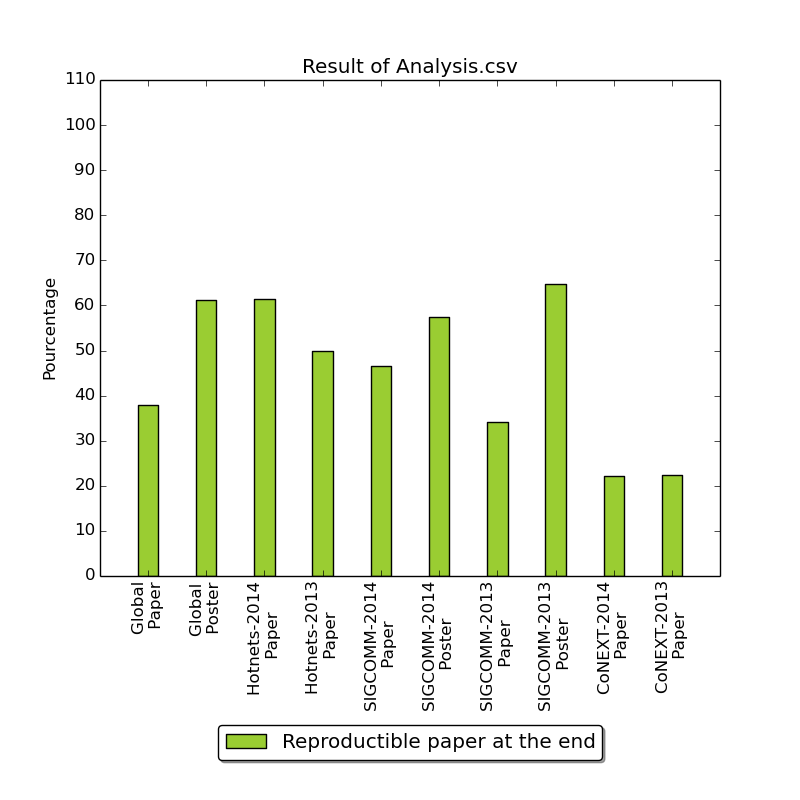
\includegraphics[width=0.7\columnwidth]{stat/final-analysis.png}} \\

        & & \\

        (a) TODO & (b) TODO & (c) TODO \\
\end{tabular}

    \caption{Result about the proportions of mail send, reason, response and at the end paper complet or not.}
     \label{f:bar_mail}
\end{figure*}




\section{Good example}

\subsection{In paper}
An experimental study of the learnability of congestion control
Network neutrality inference
Direct code execution: revisiting library OS architecture for reproducible network experiments

\subsection{In auxiliary}
Verifiable auctions for online ad exchanges
How to improve your network performance by asking your provider for worse service
TCP ex machina: computer-generated congestion control
Direct code execution: revisiting library OS architecture for reproducible network experiments




\end{document}

